
\de{ĐỀ THI HỌC KỲ I NĂM HỌC 2022-2023}{THPT Trương Vĩnh Ký - Bến Tre}
\begin{center}
	\textbf{PHẦN 1 - TRẮC NGHIỆM}
\end{center}
\Opensolutionfile{ans}[ans/ans]
\begin{ex}%[0D3Y2-3]%[Dự án đề kiểm tra HKII NH22-23-Quang Anh]%[trương Vĩnh Ký Bến Tre]
	Cho hàm số $y=x^2-3x$. Hỏi hình nào sau đây là đồ thị của hàm số đã cho?
	\choice
	{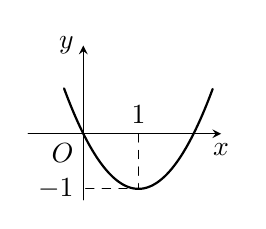
\begin{tikzpicture}[>=stealth,scale=0.7, line join=round, line cap=round]
			\draw[->] (-1,0)--(2.5,0) node [below]{$x$};
			\draw[->] (0,-1.2)--(0,1.6) node [left]{$y$};
			\node at (0,0) [below left]{$O$};
			\clip ;
			\draw[smooth,samples=300,domain=-0.35:2.35,thick] plot(\x,{(\x)^2-2*(\x)});
			\draw[dashed](1,0)node[above]{$1$}--(1,-1)--(0,-1)node[left]{$-1$};
	\end{tikzpicture}}
	{\True 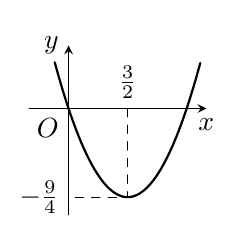
\begin{tikzpicture}[>=stealth,scale=0.5, line join=round, line cap=round]
			\draw[->] (-1,0)--(3.5,0) node [below]{$x$};
			\draw[->] (0,-2.7)--(0,1.6) node [left]{$y$};
			\node at (0,0) [below left]{$O$};
			\clip ;
			\draw[smooth,samples=300,domain=-0.35:3.35,thick] plot(\x,{(\x)^2-3*(\x)});
			\draw[dashed](3/2,0)node[above]{$\frac{3}{2}$}--(3/2,-9/4)--(0,-9/4)node[left]{$-\frac{9}{4}$};
	\end{tikzpicture}}
	{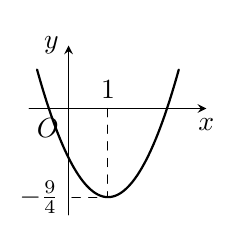
\begin{tikzpicture}[>=stealth,scale=0.5, line join=round, line cap=round]
			\draw[->] (-1,0)--(3.5,0) node [below]{$x$};
			\draw[->] (0,-2.7)--(0,1.6) node [left]{$y$};
			\node at (0,0) [below left]{$O$};
			\clip ;
			\draw[smooth,samples=300,domain=-0.8:2.8,thick] plot(\x,{(\x)^2-2*(\x)-5/4});
			\draw[dashed](1,0)node[above]{$1$}--(1,-9/4)--(0,-9/4)node[left]{$-\frac{9}{4}$};
	\end{tikzpicture}}
	{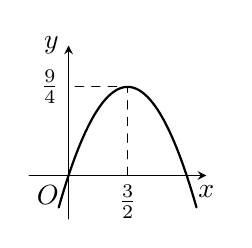
\begin{tikzpicture}[>=stealth,scale=0.5, line join=round, line cap=round]
			\draw[->] (-1,0)--(3.5,0) node [below]{$x$};
			\draw[->] (0,-1.1)--(0,3.3) node [left]{$y$};
			\node at (0,0) [below left]{$O$};
			\clip ;
			\draw[smooth,samples=300,domain=-0.25:3.25,thick] plot(\x,{-(\x)^2+3*(\x)});
			\draw[dashed](3/2,0)node[below]{$\frac{3}{2}$}--(3/2,9/4)--(0,9/4)node[left]{$\frac{9}{4}$};
	\end{tikzpicture}}
	\loigiai{
	Đồ thị hàm số $y=x^2-3x$ có $a=1>0$ và đỉnh có tọa độ là $\left(\dfrac{3}{2}; -\dfrac{9}{4}\right)$ nên ta chọn phương án parabol có bề lõm hướng lên và  đỉnh có tọa độ là $\left(\dfrac{3}{2}; -\dfrac{9}{4}\right)$.
		}
\end{ex}
\begin{ex}%[0D2Y1-2]%[Dự án đề kiểm tra HKII NH22-23-Quang Anh]%[trương Vĩnh Ký Bến Tre]
	Trong một buổi khiêu vũ có $20$ học sinh nam và $18$ học sinh nữ. Hỏi có bao nhiêu cách chọn ra một đôi nam nữ để khiêu vũ?
	\choice
	{$703$}
	{\True $360$}
	{$1406$}
	{$38$}
	\loigiai{
	Có $20$ cách chọn $1$ học sinh nam và $18$ cách chọn 1 học sinh nữ để tạo thành một cặp, nên có $360$ cách chọn một đôi nam nữ để khiêu vũ.
	}
\end{ex}
\begin{ex}%[0D2Y1-1]%[Dự án đề kiểm tra HKII NH22-23-Quang Anh]%[trương Vĩnh Ký Bến Tre]
	 Có $3$ cây bút đỏ, $4$ cây bút xanh trong một hộp bút. Hỏi có bao nhiêu cách lấy ra $1$ cây bút từ hộp bút?
	\choice
	{\True $7$}
	{$12$}
	{$4$}
	{$3$}
	\loigiai{
	Có $7$ cách lấy một cây bút bất kì từ hộp.
	}
\end{ex}
\begin{ex}%[0D2Y2-1]%[Dự án đề kiểm tra HKII NH22-23-Quang Anh]%[trương Vĩnh Ký Bến Tre]
	Có bao nhiêu cách sắp xếp $5$ học sinh thành một hàng dọc?
	\choice
	{$5$}
	{\True $120$}
	{$5^5$}
	{$24$}
	\loigiai{
	Mỗi cách xếp $5$ học sinh thành một hàng dọc là một hoán vị của $5$ phần tử.\\ Nên số cách xếp được là $5!=120$.
	}
\end{ex}
\begin{ex}%[0D4Y2-2]%[Dự án đề kiểm tra HKII NH22-23-Quang Anh]%[trương Vĩnh Ký Bến Tre]
	Tập nghiệm của bất phương trình $x^2-7x+12<0$ là
	\choice
	{$\varnothing$}
	{$(-\infty ; 3) \cup(4 ;+\infty)$}
	{\True $(3 ; 4)$}
	{$(0; 4)$}
	\loigiai{
	Tam thức bậc hai $f(x)=x^2-7x+12$ có $a=1>0, f(x)=0\Leftrightarrow \hoac{&x=3  \\ &x=4 }$.\\
	Theo định lý về dấu tam thức ta có tập nghiệm của bất phương trình đã cho là $(3; 4)$
	}
\end{ex}
\begin{ex}%[0D3Y2-1]%[Dự án đề kiểm tra HKII NH22-23-Quang Anh]%[trương Vĩnh Ký Bến Tre]
	Tọa độ đỉnh của parabol $y=-3x^2+6x-1$ là
	\choice
	{$I(2;-1)$}
	{\True $I(1; 2)$}
	{$I(-2;-25)$}
	{$I(-1;-10)$}
	\loigiai{
	Áp dụng lý thuyết với hàm số bậc hai $y=ax^2+bx+c$ thì đồ thị là parabol có đỉnh $I\left(-\dfrac{b}{2a} ;-\dfrac{\Delta}{4 a}\right)$ $\Rightarrow$ Tọa độ đỉnh là $I(1; 2)$. 
	}
\end{ex}
\begin{ex}%[0H4Y1-5]%[Dự án đề kiểm tra HKII NH22-23-Quang Anh]%[trương Vĩnh Ký Bến Tre]
	Khoảng cách từ điểm $A(7; 4)$ đến đường thẳng $d\colon 5x+3y-8=0$ có kết quả bằng
	\choice
	{$\dfrac{35}{\sqrt{34}}$}
	{\True $\dfrac{39}{\sqrt{34}}$}
	{$\dfrac{39}{4}$}
	{$\dfrac{39}{16}$}
	\loigiai{
	Áp dụng công thức khoảng cách ta có $\mathrm{d}(A; d)=\dfrac{|5\cdot7+3\cdot4-8|}{\sqrt{5^2+3^2}}=\dfrac{39}{\sqrt{34}}$.
	}
\end{ex}
\begin{ex}%[0D3Y1-2]%[Dự án đề kiểm tra HKII NH22-23-Quang Anh]%[trương Vĩnh Ký Bến Tre]
	Tìm tập xác định của hàm số $y=\dfrac{x}{x^2-2023^2}$ là 
	\choice
	{\True $\mathcal{D}=\mathbb{R}\backslash\{-2023; 2023\}$}
	{$\mathcal{D}=\mathbb{R}$}
	{$\mathcal{D}=\{-2023; 2023\}$}
	{$\mathcal{D}=\mathbb{R} \backslash\{2023\}$}
	\loigiai{
	Hàm số xác định khi $x^2-2023^2 \neq 0 \Leftrightarrow x \neq \pm 2023$.\\
	Vậy tập xác định của hàm số là $\mathcal{D}=\mathbb{R}\backslash\{-2023; 2023\}$.	
	}
\end{ex}
\begin{ex}%[0H4Y3-7]%[Dự án đề kiểm tra HKII NH22-23-Quang Anh]%[trương Vĩnh Ký Bến Tre]
	Trong mặt phẳng $Oxy$, cho phương trình parabol $(P)\colon y^2=24x$. Tiêu điểm của parabol này là
	\choice
	{$F(12; 0)$}
	{\True $F(6; 0)$}
	{$F(-6; 0)$}
	{$F(-12; 0)$}
	\loigiai{
	$(P)\colon y^2=24x \Rightarrow p=12$.\\
	Khi đó tiêu điểm của parabol là $F(6; 0)$.
	}
\end{ex}
\begin{ex}%[0D3Y2-1]%[Dự án đề kiểm tra HKII NH22-23-Quang Anh]%[trương Vĩnh Ký Bến Tre]
	Gieo một con xúc sắc cân đối, đồng chất một lần. Xác suất để xuất hiện mặt chẵn?
	\choice
	{\True $\dfrac{1}{2}$}
	{$\dfrac{1}{4}$}
	{$\dfrac{1}{6}$}
	{$\dfrac{1}{3}$}
	\loigiai{
	Gieo một con xúc sắc cân đối, đồng chất một lần.\\
	$\Rightarrow$ Số phần tử của không gian mẫu $n(\Omega)=6$.\\
	Gọi $\mathrm{A}$ là biến cố: \lq\lq Xuất hiện mặt chẵn\rq\rq $\Rightarrow n(A)=3$.\\
	Vậy xác suất của biến cố $A$ là $P(A)=\dfrac{3}{6}=\dfrac{1}{2}$.
	}
\end{ex}

\begin{ex}%[0H4Y2-1]%[Dự án đề kiểm tra HKII NH22-23-Quang Anh]%[trương Vĩnh Ký Bến Tre]
	\immini
	{
		Trong mặt phẳng $Oxy$, đường tròn như hình bên có phương trình là một trong bốn phương trình sau. Hỏi đó là phương trình nào?
		\choice
		{\True $(x-1)^2+(y+1)^2=4$}
		{$(x+1)^2+(y-1)^2=2$}
		{$(x+1)^2+(y-1)^2=4$}
		{$(x-1)^2+(y+1)^2=2$}
	}
	{
		\begin{tikzpicture}[line join=round, line cap=round,>=stealth,thick,scale=0.8]
			\draw[->] (-1.6,0)--(4,0) node[below left] {$x$};
			\draw[->] (0,-3.5)--(0,2.5) node[below left] {$y$};
			\draw (0,0) node [below left] {$O$};
			\foreach \x in {-1,3}
			\draw[thin] (\x,1pt)--(\x,-1pt) node [above] {$\x$};
			\foreach \y in {-1,1,-3}
			\draw[thin] (1pt,\y)--(-1pt,\y) node [left] {$\y$};
			\draw[dashed,thin](1,0)node[above]{$1$}--(1,-1)--(0,-1);
			\coordinate (I) at (1,-1);
			\draw[name path=c] (I) circle (2 cm);
			\foreach \i in {I}{\draw(\i) node[scale=0.9,below right]{$\i$};}
			\foreach \i in {I}{\fill[black](\i) circle (0.8pt);}
			\draw[step=1,gray,dashed,thin] (-1.7,-3.6) grid (4.2,2.6);
		\end{tikzpicture}
	}
	\loigiai{
	Từ hình vẽ ta thấy đường tròn có tâm $I(1; -1)$ và bán kính $R=2$.\\
	Vậy phương trình đường tròn là $(x-1)^2+(y+1)^2=4$.
	}
\end{ex}
\begin{ex}%[0H4Y1-4]%[Dự án đề kiểm tra HKII NH22-23-Quang Anh]%[trương Vĩnh Ký Bến Tre]
	Gọi $\varphi$ là góc giữa hai đường thẳng $d_1\cdot -x+2y-3=0$ và $d_2\colon 2x-y+7=0$. Tính $\cos \varphi$.
	\choice
	{$\cos \varphi=-\dfrac{4}{5}$}
	{$\cos \varphi=0$}
	{$\cos \varphi=\dfrac{4}{25}$}
	{\True $\cos \varphi=\dfrac{4}{5}$}
	\loigiai{
	$d_1\colon -x+2 y-3=0$ có vectơ pháp tuyến $\vec{n}=(-1; 2)$.\\
	$d_2\colon 2x-y+7=0$ có vectơ pháp tuyến $\vec{n^\prime}=(2; -1)$.\\
	Góc giữa hai đường thẳng $d_1$ và $d_2$ là $\cos \varphi=\dfrac{\left|\vec{n} \cdot \overrightarrow{n^{\prime}}\right|}{|\vec{n} \cdot|\left|\overrightarrow{n^{\prime}}\right|}=\dfrac{|-2-2|}{\sqrt{5} \cdot \sqrt{5}}=\dfrac{4}{5}$.
	}
\end{ex}
\begin{ex}%[0D2Y1-2]%[Dự án đề kiểm tra HKII NH22-23-Quang Anh]%[trương Vĩnh Ký Bến Tre]
	\immini
	{
	Mã xác thực (OTP - One Time Password) do một ngân hàng gửi vào điện thoại của khách hàng cho mỗi lần giao là một dãy 6 kí tự từ các chữ số từ $0$ đến $9$. Có thể tạo ra bao nhiêu mã xác thực khác nhau như vậy? 
	}
	{%Khaibaothemgoi \usepackage{boxedminipage}
		\begin{boxedminipage}[t]{5.5cm}
			\textbf{\texttt{Mã OTP xác thực giao dịch là 712892, hiệu lực trong 1 phút$\ldots$}}
		\end{boxedminipage}
	}
	\choice
	{$151200$}
	{$136080$}
	{\True $1000000$}
	{$900000$}
	\loigiai{
	Mỗi kí tự trong dãy đều có $10$ cách chọn nên theo quy tắc nhân có thể tạo ra $10^6$ dãy.
	}
\end{ex}
\begin{ex}%[0H4Y1-1]%[Dự án đề kiểm tra HKII NH22-23-Quang Anh]%[trương Vĩnh Ký Bến Tre]
	Trong mặt phẳng $Oxy$, đường thẳng qua điểm $M(4; 5)$ và nhận $\vec{u}=(2; 3)$ làm véc tơ chỉ phương có phương trình tham số là
	\choice
	{$\heva{&x=2+4t \\ &y=3+5t}(t \in \mathbb{R})$}
	{\True $\heva{&x=4+2t \\ &y=5+3t}(t \in \mathbb{R})$}
	{$\heva{&x=4+5t \\ &y=2+3t}(t \in \mathbb{R})$}
	{$\heva{&x=2+t \\ &y=5+3t}(t \in \mathbb{R})$}
	\loigiai{
	 Đường thẳng qua điểm $M(4 ; 5)$ và nhận $\vec{u}=(2 ; 3)$ làm véc-tơ chỉ phương có phương trình tham số là $\heva{&x=4+2t \\& y=5+3t}(t \in \mathbb{R})$.
	}
\end{ex}

\begin{ex}%[0D2Y3-1]%[Dự án đề kiểm tra HKII NH22-23-Quang Anh]%[trương Vĩnh Ký Bến Tre]
	Kết quả của khai triển $(x-y)^4$ là
	\choice
	{\True $x^4-4 x^3y+6 x^2y^2-4 xy^3+y^4$}
	{$x^4-x^3 y+x^2 y^2-x y^3+y^4$}
	{$x^4-4 x^3 y+12 x^2 y^2-24 x y^3+12 y^4$}
	{$x^4+4 x^3 y+6 x^2 y^2+4 x y^3+y^4$}
	\loigiai{Ta có 
		\allowdisplaybreaks
		\begin{eqnarray*}
			(x-y)^4&=&\mathrm{C}_4^0 x^4+\mathrm{C}_4^1 x^3(-y)+\mathrm{C}_4^2 x^2(-y)^2+\mathrm{C}_4^3 x(-y)^3+\mathrm{C}_4^4(-y)^4\\
			&=&x^4-4 x^3 y+6 x^2 y^2-4 x y^3+y^4.
		\end{eqnarray*}
	}
\end{ex}

\begin{ex}%[0H4Y1-1]%[Dự án đề kiểm tra HKII NH22-23-Quang Anh]%[trương Vĩnh Ký Bến Tre]
	Trong mặt phẳng $Oxy$, cho đường thẳng $\Delta\colon\heva{&x=5+2 t \\& y=3-t}(t \in \mathbb{R})$. Một véc-tơ chỉ phương của đường thẳng $\Delta$ có tọa độ là
	\choice
	{$(2; 1)$}
	{\True $(2; -1)$}
	{$(1; 2)$}
	{$(5; 3)$}
	\loigiai{
	Đường thẳng $\Delta\colon\heva{&x=5+2t \\ &y=3-t}(t \in \mathbb{R})$ có một véc-tơ chỉ phương là $\vec{u}=(2 ;-1)$.
	}
\end{ex}
\begin{ex}%[0H4Y2-1]%[Dự án đề kiểm tra HKII NH22-23-Quang Anh]%[trương Vĩnh Ký Bến Tre]
	Trong mặt phẳng $Oxy$, cho đường tròn $(C)\colon x^2+y^2-4x+6y-1=0$. Tìm tọa độ tâm của đường tròn đã cho.
	\choice
	{$(-2; 3)$}
	{$(-4; 6)$}
	{\True $(2;-3)$}
	{$(4;-6)$}
	\loigiai{
	Tọa độ tâm $I$ là $\heva{&x_I=\dfrac{-4}{-2}=2 \\& y_I=\dfrac{6}{-2}=-3}\Rightarrow I(2;-3)$.
	}
\end{ex}
\begin{ex}%[0H4Y3-1]%[Dự án đề kiểm tra HKII NH22-23-Quang Anh]%[trương Vĩnh Ký Bến Tre]
	Trong mặt phẳng $Oxy$, cho phương trình elip $(E)\colon \dfrac{x^2}{17}+\dfrac{y^2}{9}=1$. Tiêu cự của $(E)$ bằng
	\choice
	{\True $4\sqrt{2}$}
	{$\sqrt{26}$}
	{$2\sqrt{26}$}
	{$2\sqrt{2}$}
	\loigiai{
	Từ phương trình elip ta có $a=\sqrt{17}; b=3$.\\
	Vây tiêu cự là $2c=2\sqrt{a^2-b^2}=4\sqrt{2}$.
	}
\end{ex}
\begin{ex}%[Dự án đề kiểm tra HKII NH22-23-Quang Anh]%[trương Vĩnh Ký Bến Tre]
	Trong mặt phẳng $Oxy$, cho đường tròn $(C)\colon(x-2)^2+(y+5)^2=17$. Tiếp tuyến với $(C)$ tại điềm $A(3;-1)$ có phương trình là
	\choice
	{\True $x+4y+1=0$}
	{$-x+4y+7=0$}
	{$x+4y+18=0$}
	{$x-6y-9=0$}
	\loigiai{
	$(C)$ có tâm $I(2;-5)$ và bán kính $R=\sqrt{17}$.
	Tiếp tuyến cần tìm có một véc-tơ pháp tuyến là $\vec{IA}=(1; 4)$ và đi qua điểm $A(3;-1)$. Suy ra có phương trình là $$1(x-3)+4(y+1)=0 \Leftrightarrow x+4 y+1=0.$$
	}
\end{ex}
\begin{ex}%[0D4Y1-2]%[Dự án đề kiểm tra HKII NH22-23-Quang Anh]%[trương Vĩnh Ký Bến Tre]
	\immini
	{	Cho hàm số $f(x)=ax^2+bx+c$ có đồ thị như hình bên. Tìm tất cả giá trị của $x$ để $f(x)<0$.
		\choice
		{$x\in(-\infty; 1) \cup(3;+\infty)$}
		{\True $x\in(1; 3)$}
		{$x\in(0 ; 2)$}
		{$x\in(-1 ; 0)$}
	}
	{
		\begin{tikzpicture}[line join=round, line cap=round,>=stealth,thick]
			\tikzset{every node/.style={scale=0.6}}
			\draw[->] (-0.5,0)--(4.5,0) node[below left] {$x$};
			\draw[->] (0,-1.1)--(0,3.1) node[below left] {$y$};
			\draw (0,0) node [below left] {$O$};
			\foreach \x in {1,2,3,4}
			\draw[thin] (\x,1pt)--(\x,-1pt) node [below] {$\x$};
			\foreach \y in {-1,1,2}
			\draw[thin] (1pt,\y)--(-1pt,\y) node [left] {$\y$};
			\begin{scope}
				\clip (-1,-2) rectangle (5,3);
				\draw[samples=200,domain=0.2:3.8,smooth,variable=\x] plot (\x,{1*(\x)^2+-4*(\x)+3});
			\end{scope}
		\end{tikzpicture}
	}
	
	\loigiai{
	Vì $f(x)<0$ nên ta tìm các giá trị $x$ ứng với phần đồ thị nằm phía dưới trục hoành.\\ Vậy $x\in(1 ; 3)$.
	}
\end{ex}

\begin{ex}%[0D3Y1-1]%[Dự án đề kiểm tra HKII NH22-23-Quang Anh]%[trương Vĩnh Ký Bến Tre]
	Hàm số mô tả sự phụ thuộc của $y$ (số tiền phải trả, tính bằng nghìn đồng) vào $x$ (lượng điện tiêu thu tính bằng kWh) trên từng khoảng giá trị $x$, được cho bởi công thức sau:
	$$
	y= \begin{cases}1{,}678 x & \text{Nếu}\; 0 \leq x \leq 50 \\ 1{,}734 x-2{,}8 & \text{Nếu}\; 0<x \leq 100 \\ 2{,}014 x-30{,}8 &\text{Nếu}\; 100<x \leq 200 \\ 2{,}536 x-135{,}2 &\text{Nếu}\; 200<x \leq 300 \\ 2{,}834 x-224{,}6 &\text{Nếu}\; 300<x \leq 400 \\ 2{,}927 x-261{,}8 & \text{Nếu}\; x>400\end{cases}
	$$
	Ông An tháng thứ nhất sài hết $90$kWh điện, tháng thứ hai sài hết $120$kWh điện. Theo công thức trên số tiền ông An phải trà sau hai tháng gần nhất với kết quả nào sau đây?
	\choice
	{\True $364$ nghìn đồng}
	{$361$ nghìn đồng}
	{$392$ nghìn đồng}
	{$352$ nghìn đồng}
	\loigiai{
	Tháng thứ nhất sài hết $90$kWh nên số tiền phải trà là: $1{,}734\cdot90-2{,}8=153{,}26$ nghìn đồng.\\
	Tháng hai sài hết $120$kWh nên số tiền phải trà là: $2{,}014\cdot120-30{,}8=210{,}88$ nghìn đồng.\\
	Vậy ông An phải trả sau hai tháng là: $153{,}26+210{,}88=364{,}14$ nghìn đồng.	
	}
\end{ex}
\begin{ex}%[0D3B2-1]%[Dự án đề kiểm tra HKII NH22-23-Quang Anh]%[trương Vĩnh Ký Bến Tre]
	Biết Parabol $(P)\colon y=ax^2+bx+c$ đi qua điểm $A(2; 1)$ và $B(-3; 5)$. Tính giá trị biểu thức $S=44a-8b+6c+3$.
	\choice
	{$S=6$}
	{\True $S=25$}
	{$S=-15$}
	{$S=22$}
	\loigiai{
	Parabol $(P)\colon y=ax^2+bx+c$ đi qua điểm $A(2; 1)$ và $B(-3; 5)$ suy ra ta có:
	$$
	\heva{& 
		a\cdot 2^2+ b\cdot 2+c=1\\& a\cdot (-3)^2+b\cdot(-3)+c=5}\Leftrightarrow \heva{&4a+2b+c=1\\&9a-3b+c=5}\Leftrightarrow \heva{&8a+4b+2c=2 \\&
		36a-12b+4c=20.}
	$$
	Cộng vế với vế của phương trình (1) và (2) ta được: $S=44 a-8 b+6 c+3=25$.
	}
\end{ex}
\begin{ex}%[0D4B2-3]%[Dự án đề kiểm tra HKII NH22-23-Quang Anh]%[trương Vĩnh Ký Bến Tre]
	Bác Hùng dùng $40$m lưới thép gai rào thành một mảnh vườn hình chữ nhật để trồng rau. Gọi $x$ (m) là kích thước chiều rộng của hình chữ nhật. Để diện tích mảnh vườn nói trên không nhỏ hơn $91\mathrm{~m}^2$ thì thì $x$ nhận giá trị nào sau đây?
	\choice
	{$x\in[6; 10]$}
	{$x\in[7; 13]$}
	{\True  $x\in[7; 10]$}
	{$x\in[6; 13]$}
	\loigiai{
	Theo đề chiều rộng của hình chữ nhật là: $x$ (m).\\
	Chiều dài của hình chữ nhật là $20-x$ (m), điều kiện $20-x\geq x\Rightarrow x\leq 10 $.\\
	Theo đề bài ta có $x\cdot(20-x) \geq 91 \Leftrightarrow-x^2+20 x-91 \geq 0 \Leftrightarrow 7 \leq x \leq 13$.\\
	So với điều kiện suy ra $x\in[7; 10]$.	
	}
\end{ex}
\begin{ex}%[0D3B2-4]%[Dự án đề kiểm tra HKII NH22-23-Quang Anh]%[trương Vĩnh Ký Bến Tre]
	Một lô hàng $20$ sản phẩm trong đó có $4$ phế phẩm. Lấy tùy ý $6$ sản phẩm từ lô hàng đó. Tính xác suất để $6$ sản phẩm đó có không quá một phế phẩm.
	\choice
	{$\dfrac{91}{285}$}
	{\True $\dfrac{637}{969}$}
	{$\dfrac{7}{9}$}
	{$\dfrac{91}{323}$}
	\loigiai{
	Không gian mẫu $\Omega$: \lq\lq Lấy 6 sản phẩm trong 20 sản phẩm\rq\rq \,suy ra $n(\Omega)=\mathrm{C}_{20}^6$.\\
	Biến cố $A$: \lq\lq Lấy 6 sản phẩm có không quá một phẩm\rq\rq\, suy ra $n(A)=\mathrm{C}_{16}^5 \cdot \mathrm{C}_4^1+\mathrm{C}_{16}^6$.\\
	Vậy xác suất để $6$ sản phẩm đó có không quá một phế phẩm là:
	$$
	\mathrm{P}(A)=\dfrac{n(A)}{n(\Omega)}=\dfrac{\mathrm{C}_{16}^5 \cdot \mathrm{C}_4^1+\mathrm{C}_{16}^6}{\mathrm{C}_{20}^6}=\dfrac{637}{969}.
	$$
	}
\end{ex}
\begin{ex}%[0D3B2-3]%[Dự án đề kiểm tra HKII NH22-23-Quang Anh]%[trương Vĩnh Ký Bến Tre]
	Một nhóm công nhân gồm $15$ nam và $5$ nữ. Người ta muốn chọn từ nhóm ra $5$ người để lập thành một tổ công tác gồm một tổ trưởng là nam, một tổ phó là nam và $3$ người còn lại có ít nhất một nữ. Hỏi có bao nhiêu cách lập tổ công tác?
	\choice
	{\True $111300$}
	{$233355$}
	{$109200$}
	{$112342$}
	\loigiai{
	Lấy $2$ nam ra làm tổ trưởng và tổ phó là chỉnh hợp chập $2$ của $15$ phần tử. Lúc này $3$ người còn lại có ít nhất một nữ sẽ xảy ra các trường hợp sau:
	\begin{itemize}
		\item \textbf{TH1.} $2$ nam và $1$ nữ.
		\item \textbf{TH2.} $1$ nam và $2$ nữ.
		\item \textbf{TH3.} $3$ nữ.
	\end{itemize}
	Theo đề ta có số cách lập một tổ công tác là $$n(\Omega)=\mathrm{A}_{15}^2 \cdot \mathrm{C}_{13}^2 \cdot \mathrm{C}_5^1+\mathrm{A}_{15}^2 \cdot \mathrm{C}_{13}^1 \cdot \mathrm{C}_5^2+\mathrm{A}_{15}^2 \cdot \mathrm{C}_5^3=111300.$$
	}
\end{ex}

\Closesolutionfile{ans}
%\begin{center}
%	\textbf{ĐÁP ÁN}
%	\inputansbox{10}{ans/ans}	
%\end{center}
\begin{center}
	\textbf{PHẦN 2 - TỰ LUẬN}
\end{center}

\begin{bt}%[0D3B2-3]%[Dự án đề kiểm tra HKI NH22-23-Thy Nguyen Vo Diem]%[THPT Trương Vĩnh Ký - Bến Tre]
	Cho hàm số $y=-2x^2+6x$ có đồ thị $(P)$.
	\begin{listEX}[1]
		\item Vẽ đồ thị $(P)$.
		\item Tìm toạ độ giao điểm của $(P)$ với trục hoành.
	\end{listEX}
	\loigiai{
		\begin{listEX}
			\item Vẽ đồ thị $(P)$
			\begin{itemize}
				\item Tọa độ đỉnh $S\left(\dfrac{3}{2};\dfrac{9}{2}\right)$.
				\item Trục đối xứng $x=\dfrac{3}{2}$.
				\item Bảng giá trị
				\begin{center}
					\begin{tabular}{|c|c|c|c|c|c|c|}
						\hline
						$x$ & $0$ &$1$ & $\tfrac{3}{2}$&$2$ &$3$\\
						\hline
						$y=-2x^2+6x$ & $0$ & $4$  &$\tfrac{9}{2}$  & $2$  & $0$\\
						\hline
					\end{tabular}
				\end{center}
				\item Đồ thị
				\begin{center}
					\begin{tikzpicture}[line join=round, line cap=round,>=stealth,thick]
						\def \xmin{-1}
						\def \xmax{4.55}
						\def \ymin{-1}
						\def \ymax{5}
						\draw[->] (\xmin,0)--(\xmax,0) node[below left] {$x$};
						\draw[->] (0,\ymin)--(0,\ymax) node[below right] {$y$};
						\draw (0,0) node [below right] {$O$};
						%%Vẽ các điểm trên 2 hệ trục
						\path (1,0) node [below left] {$1$} 
						(1.5,0) node[below left] {$\tfrac{3}{2}$}
						(2,0) node [below] {$2$}
						(3,0) node [below left] {$3$}
						(0,4.5) node[left] {$\tfrac{9}{2}$}
						(0,4) node[left] {$4$};
						%%Vẽ đỉnh và trục đối xứng
						\draw[dashed,thin](1.5,4.5)--(0,4.5);
						\draw[dashed, thin] (1.5,\ymin)--(1.5,\ymax);
						\draw[dashed, thin] (1,0)--(1,4) (2,0)--(2,4)--(0,4);
						\begin{scope}
							\clip (\xmin+0.01,\ymin+0.01) rectangle (\xmax-0.01,\ymax-0.01);
							\draw[samples=350,domain=\xmin+0.01:\xmax-0.01,smooth,variable=\x] plot (\x,{-2*(\x)^2+6*(\x)});
						\end{scope}
					\end{tikzpicture}
					
				\end{center}
			\end{itemize}
			\item Tọa độ giao điểm của $(P)$ và trục hoành là nghiệm hệ phương trình
			$$\heva{&y=-2x^2+6x\\&y=0} \Leftrightarrow \heva{&-2x^2+6x =0 \\ & y=0} \Leftrightarrow \heva{&\hoac{&x=0\\&x=3} \\&y=0.}$$
			Vậy tọa độ giao điểm của $(P)$ và trục hoành là $(0;0)$, $(3;0)$.
		\end{listEX}
	}
\end{bt}

\begin{bt}%[0D4B3-1]%[Dự án đề kiểm tra HKI NH22-23-Thy Nguyen Vo Diem]%[THPT Trương Vĩnh Ký - Bến Tre]
	Giải phương trình sau $\sqrt{3x^2+5x-6}=x+3$.
	\loigiai{
		Ta có 
		\begin{eqnarray*}
			&& \sqrt{3x^2+5x-6}=x+3 \\
			&\Rightarrow & 3x^2+5x-6=x^2+6x+9\\
			&\Rightarrow& 2x^2-x-15=0 \\
			&\Rightarrow& \hoac{&x=3\\&x=-\dfrac{5}{2}.}
		\end{eqnarray*}	
		Thử lại nhận $x=3$, $x=-\dfrac{5}{2}$.\\
		Vậy tập nghiệm phương trình là $S=\left\{ 3; -\dfrac{5}{2}\right\}$.
	}
\end{bt}

\begin{bt}%[0H4Y2-2]
	Trong mặt phẳng $Oxy$, cho hai điểm $M(3;2)$, $N(1;-4)$. Hãy viết phương trình đường tròn đường kính $MN$.
	\loigiai{
		Gọi $I$ là tâm của đường tròn. Suy ra, $I$ là trung điểm của $MN$.\\
		Do đó $I(2;-1)$.\\
		Đường tròn cần tìm có tâm $I(2;-1)$ và qua $M(3;2)$ có dạng
		$$(x-2)^2+(y+1)^2=(3-2)^2+(2+1)^2 \Leftrightarrow (x-2)^2+(y+1)^2=10.$$	
	}
\end{bt}

\begin{bt}%[0D2B1-4]%[Dự án đề kiểm tra HKI NH22-23-Thy Nguyen Vo Diem]%[THPT Trương Vĩnh Ký - Bến Tre]
	Một nhóm học sinh gồm $10$ học sinh nam và $7$ học sinh nữ. Từ nhóm này, hỏi có bao nhiêu cách chọn ra một nhóm nhỏ gồm $4$ học sinh sao cho nhóm có đủ cả nam và nữ.
	\loigiai{
		\begin{itemize}
			\item Chọn $4$ học sinh bất kì có $\mathrm{C}_{17}^4$ cách.
			\item Chọn $4$ học sinh nam có $\mathrm{C}_{10}^4$ cách.
			\item Chọn $4$ học sinh nữ có $\mathrm{C}_7^4$ cách.
		\end{itemize}
		Vậy có $\mathrm{C}_{17}^4 - \mathrm{C}_{10}^4 - \mathrm{C}_7^4 = 2135$.
	}
\end{bt}

\begin{bt}%[0D2B2-3]%[Dự án đề kiểm tra HKI NH22-23-Thy Nguyen Vo Diem]%[THPT Trương Vĩnh Ký - Bến Tre]
	Một biển số xe có mã $71-$C$4$ ở phần trên, phần dưới là một dãy gồm $5$ chữ số chọn từ các số $0$ đến $9$. Hỏi có thể tạo ra được bao nhiêu biển số xe thỏa điều kiện: Trong dãy $5$ chữ số ở phần dưới, hai chữ số cuối phải là $99$ và ba chữ số đầu phải khác nhau?
	\loigiai{
		Gọi dãy $5$ số ở phần dưới dạng $\overline{a_1a_2a_399}$. Điều kiện: $a_i\neq a_j$ với $i\leq j$ và $i$, $j \in \{1;2;3\}$.\\
		Mỗi cách chọn $a_1$, $a_2$, $a_3$ là một chỉnh hợp $3$ phần tử của $10$. Do đó, số cách chọn là $\mathrm{A}_{10}^3$.\\
		Vậy số biển số xe thỏa điều kiện đã cho là $\mathrm{A}_{10}^3 = 720$.
	}
\end{bt}

\begin{bt}%[0D3K2-5]%[Dự án đề kiểm tra HKI NH22-23-Thy Nguyen Vo Diem]%[THPT Trương Vĩnh Ký - Bến Tre]
	\immini{Một quân vua được đặt trên một ô giữa
		bàn cờ vua. Mỗi bước di chuyển, quân vua được chuyển
		sang một ô khác chung cạnh hoặc chung đỉnh với ô đang
		đứng (xem hình minh họa). Bạn An di chuyển quân vua
		ngẫu nhiên $3$ bước. Tính xác suất để sau $3$ bước đi quân
		vua trở về ô xuất phát?
	}{
		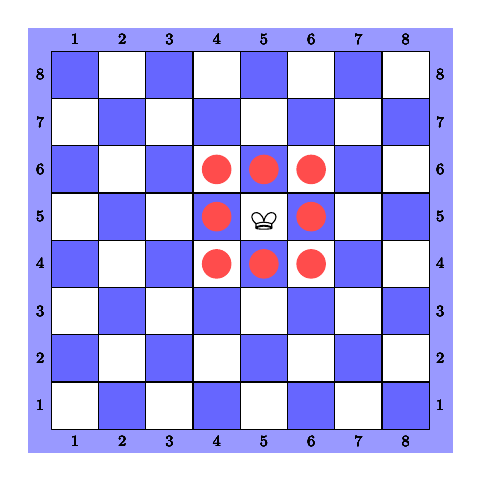
\begin{tikzpicture}[font=\footnotesize, line join=round, line cap=round, >=stealth]
			% Vẽ pic vua
			\begin{scope}[scale=.6]
				\tikzset{vua/.pic={
						\def\a{1}
						\draw([shift={(0,-\a/4)}]-\a/2,0)--(-\a/2,0)..controls ++ (140:1) and ++(100:1)..(0,0.15)..controls ++(80:1) and ++(40:1)..(\a/2,0)--++(-90:\a/4)..controls++(-30:0.25) and++(-150:0.25)..(-\a/2,-\a/4);
						\foreach \d in {0,\a/5,\a/4}{
							\draw[shift={(0,-\d)}](-\a/2,0)--(-\a/2,0)..controls++(20:0.15)and++(180:0.15)..(0,0.1)..controls++(0:0.15) and++(160:0.15)..(\a/2,0);
				}}}
				%Vẽ pic hình tròn đỏ
				\tikzset{vitri/.pic={
						\def\a{0.75}
						\draw[fill=red!70,draw=none,scale=.5](0,0) circle(\a/2);
				}}
				\fill[blue!40](-0.5,-0.5)rectangle(8.5,8.5);
				%Tô màu ô vuông
				\foreach \i in{0,1,...,7}
				\foreach \j in{0,1,...,7}
				{
					\pgfmathparse{mod(\i+\j,2)? "blue!60": "white"}
					\fill[\pgfmathresult,draw=black](\i,\j)rectangle(\i+1,\j+1);
					\pgfmathsetmacro{\k}{int(\j+1)}
					\path(0,\j+0.5)node[scale=.7,left]{\k}(8,\j+0.5)node[scale=.7,right]{\k}(\j+0.5,0)node[scale=.7,below]{\k}(\j+0.5,8)node[scale=.7,above]{\k};
				}
				%Nhập tọa độ vị trí của vua
				\path(4.5,4.35)pic[scale=0.2]{vua};
				% Nhập vị trí các ô tròn
				\foreach \x/\y in{5/5,4/5,3/5,3/4,3/3,4/3,5/3,5/4}
				\path[shift={(0.5,0.5)}](\x,\y)pic{vitri};
			\end{scope} 
		\end{tikzpicture}
	}
	\loigiai{
		Gọi $\Omega$ là không gian mẫu. Từ vị trí của quân vua, cứ mỗi bước sẽ có $8$ vị trí mà quân vua có thể đi. Do đó $|\Omega|=8^3=512$.\\
		Gọi $A$ là biến cố: "sau $3$ bước quân vua về ô xuất phát".\\
		\begin{itemize}
			\item TH1: đi theo hình tam giác vuông cân tại đỉnh vua ban đầu $4\cdot 2 = 8$ cách.
			\begin{center}
				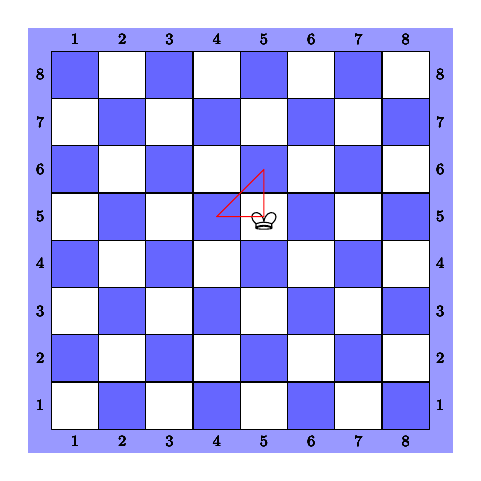
\begin{tikzpicture}[font=\footnotesize, line join=round, line cap=round, >=stealth]
					% Vẽ pic vua
					\begin{scope}[scale=.6]
						\tikzset{vua/.pic={
								\def\a{1}
								\draw([shift={(0,-\a/4)}]-\a/2,0)--(-\a/2,0)..controls ++ (140:1) and ++(100:1)..(0,0.15)..controls ++(80:1) and ++(40:1)..(\a/2,0)--++(-90:\a/4)..controls++(-30:0.25) and++(-150:0.25)..(-\a/2,-\a/4);
								\foreach \d in {0,\a/5,\a/4}{
									\draw[shift={(0,-\d)}](-\a/2,0)--(-\a/2,0)..controls++(20:0.15)and++(180:0.15)..(0,0.1)..controls++(0:0.15) and++(160:0.15)..(\a/2,0);
						}}}
						%Vẽ pic hình tròn đỏ
						\tikzset{vitri/.pic={
								\def\a{0.75}
								\draw[fill=red!70,draw=none,scale=.5](0,0) circle(\a/2);
						}}
						\fill[blue!40](-0.5,-0.5)rectangle(8.5,8.5);
						%Tô màu ô vuông
						\foreach \i in{0,1,...,7}
						\foreach \j in{0,1,...,7}
						{
							\pgfmathparse{mod(\i+\j,2)? "blue!60": "white"}
							\fill[\pgfmathresult,draw=black](\i,\j)rectangle(\i+1,\j+1);
							\pgfmathsetmacro{\k}{int(\j+1)}
							\path(0,\j+0.5)node[scale=.7,left]{\k}(8,\j+0.5)node[scale=.7,right]{\k}(\j+0.5,0)node[scale=.7,below]{\k}(\j+0.5,8)node[scale=.7,above]{\k};
						}
						%Nhập tọa độ vị trí của vua
						\path(4.5,4.35)pic[scale=0.2]{vua};
						% Nhập vị trí các ô tròn
						\draw[color=red] (4.5,4.5)--(4.5,5.5)--(3.5,4.5)--(4.5,4.5);
					\end{scope} 
				\end{tikzpicture}
			\end{center}
			\item TH2: đi theo hình tam giác vuông cân tại đỉnh khác vua có $8\cdot 2= 16$ cách
			\begin{center}
				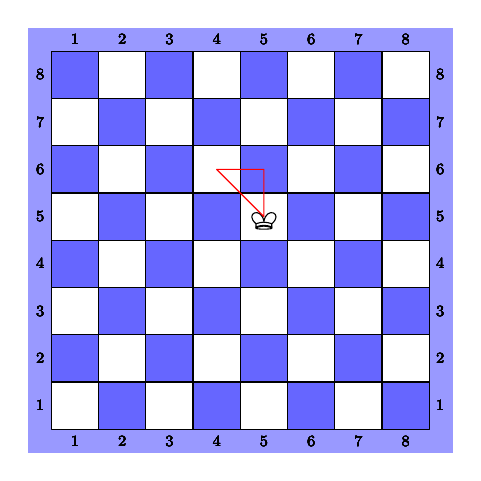
\begin{tikzpicture}[font=\footnotesize, line join=round, line cap=round, >=stealth]
					% Vẽ pic vua
					\begin{scope}[scale=.6]
						\tikzset{vua/.pic={
								\def\a{1}
								\draw([shift={(0,-\a/4)}]-\a/2,0)--(-\a/2,0)..controls ++ (140:1) and ++(100:1)..(0,0.15)..controls ++(80:1) and ++(40:1)..(\a/2,0)--++(-90:\a/4)..controls++(-30:0.25) and++(-150:0.25)..(-\a/2,-\a/4);
								\foreach \d in {0,\a/5,\a/4}{
									\draw[shift={(0,-\d)}](-\a/2,0)--(-\a/2,0)..controls++(20:0.15)and++(180:0.15)..(0,0.1)..controls++(0:0.15) and++(160:0.15)..(\a/2,0);
						}}}
						%Vẽ pic hình tròn đỏ
						\tikzset{vitri/.pic={
								\def\a{0.75}
								\draw[fill=red!70,draw=none,scale=.5](0,0) circle(\a/2);
						}}
						\fill[blue!40](-0.5,-0.5)rectangle(8.5,8.5);
						%Tô màu ô vuông
						\foreach \i in{0,1,...,7}
						\foreach \j in{0,1,...,7}
						{
							\pgfmathparse{mod(\i+\j,2)? "blue!60": "white"}
							\fill[\pgfmathresult,draw=black](\i,\j)rectangle(\i+1,\j+1);
							\pgfmathsetmacro{\k}{int(\j+1)}
							\path(0,\j+0.5)node[scale=.7,left]{\k}(8,\j+0.5)node[scale=.7,right]{\k}(\j+0.5,0)node[scale=.7,below]{\k}(\j+0.5,8)node[scale=.7,above]{\k};
						}
						%Nhập tọa độ vị trí của vua
						\path(4.5,4.35)pic[scale=0.2]{vua};
						% Nhập vị trí các ô tròn
						\draw[color=red] (4.5,4.5)--(4.5,5.5)--(3.5,5.5)--(4.5,4.5);
					\end{scope} 
				\end{tikzpicture}
			\end{center}
		\end{itemize}
		Do đó $|A|=8+16=24$ cách.\\
		Xác suất để sau $3$ bước đi quân vua về ô xuất phát là $$P(A)=\dfrac{|A|}{|\Omega|}=\dfrac{24}{512}=\dfrac{3}{64}.$$
	}
\end{bt}